\documentclass[a4paper,12pt]{article}

% defining margin for the document
\usepackage[margin=1.00in]{geometry}

% these packages are used for images
\usepackage{graphicx}

\title{Problem 4: Debugger}
\author{Saraswati Saud \\
Student ID: 40115097}
\date{}
\begin{document}
\maketitle
\section{Eclipse Debugger}
    Eclipse allows us to start a Java program in Debug mode. So, I am using the inbuilt Eclipse debugger for debugging my code. I have chosen Eclipse debugger mainly for two reasons. First, it is free and open source. Second, because of its familiarity as I have been using Eclipse IDE for a very long time.\\ \\
    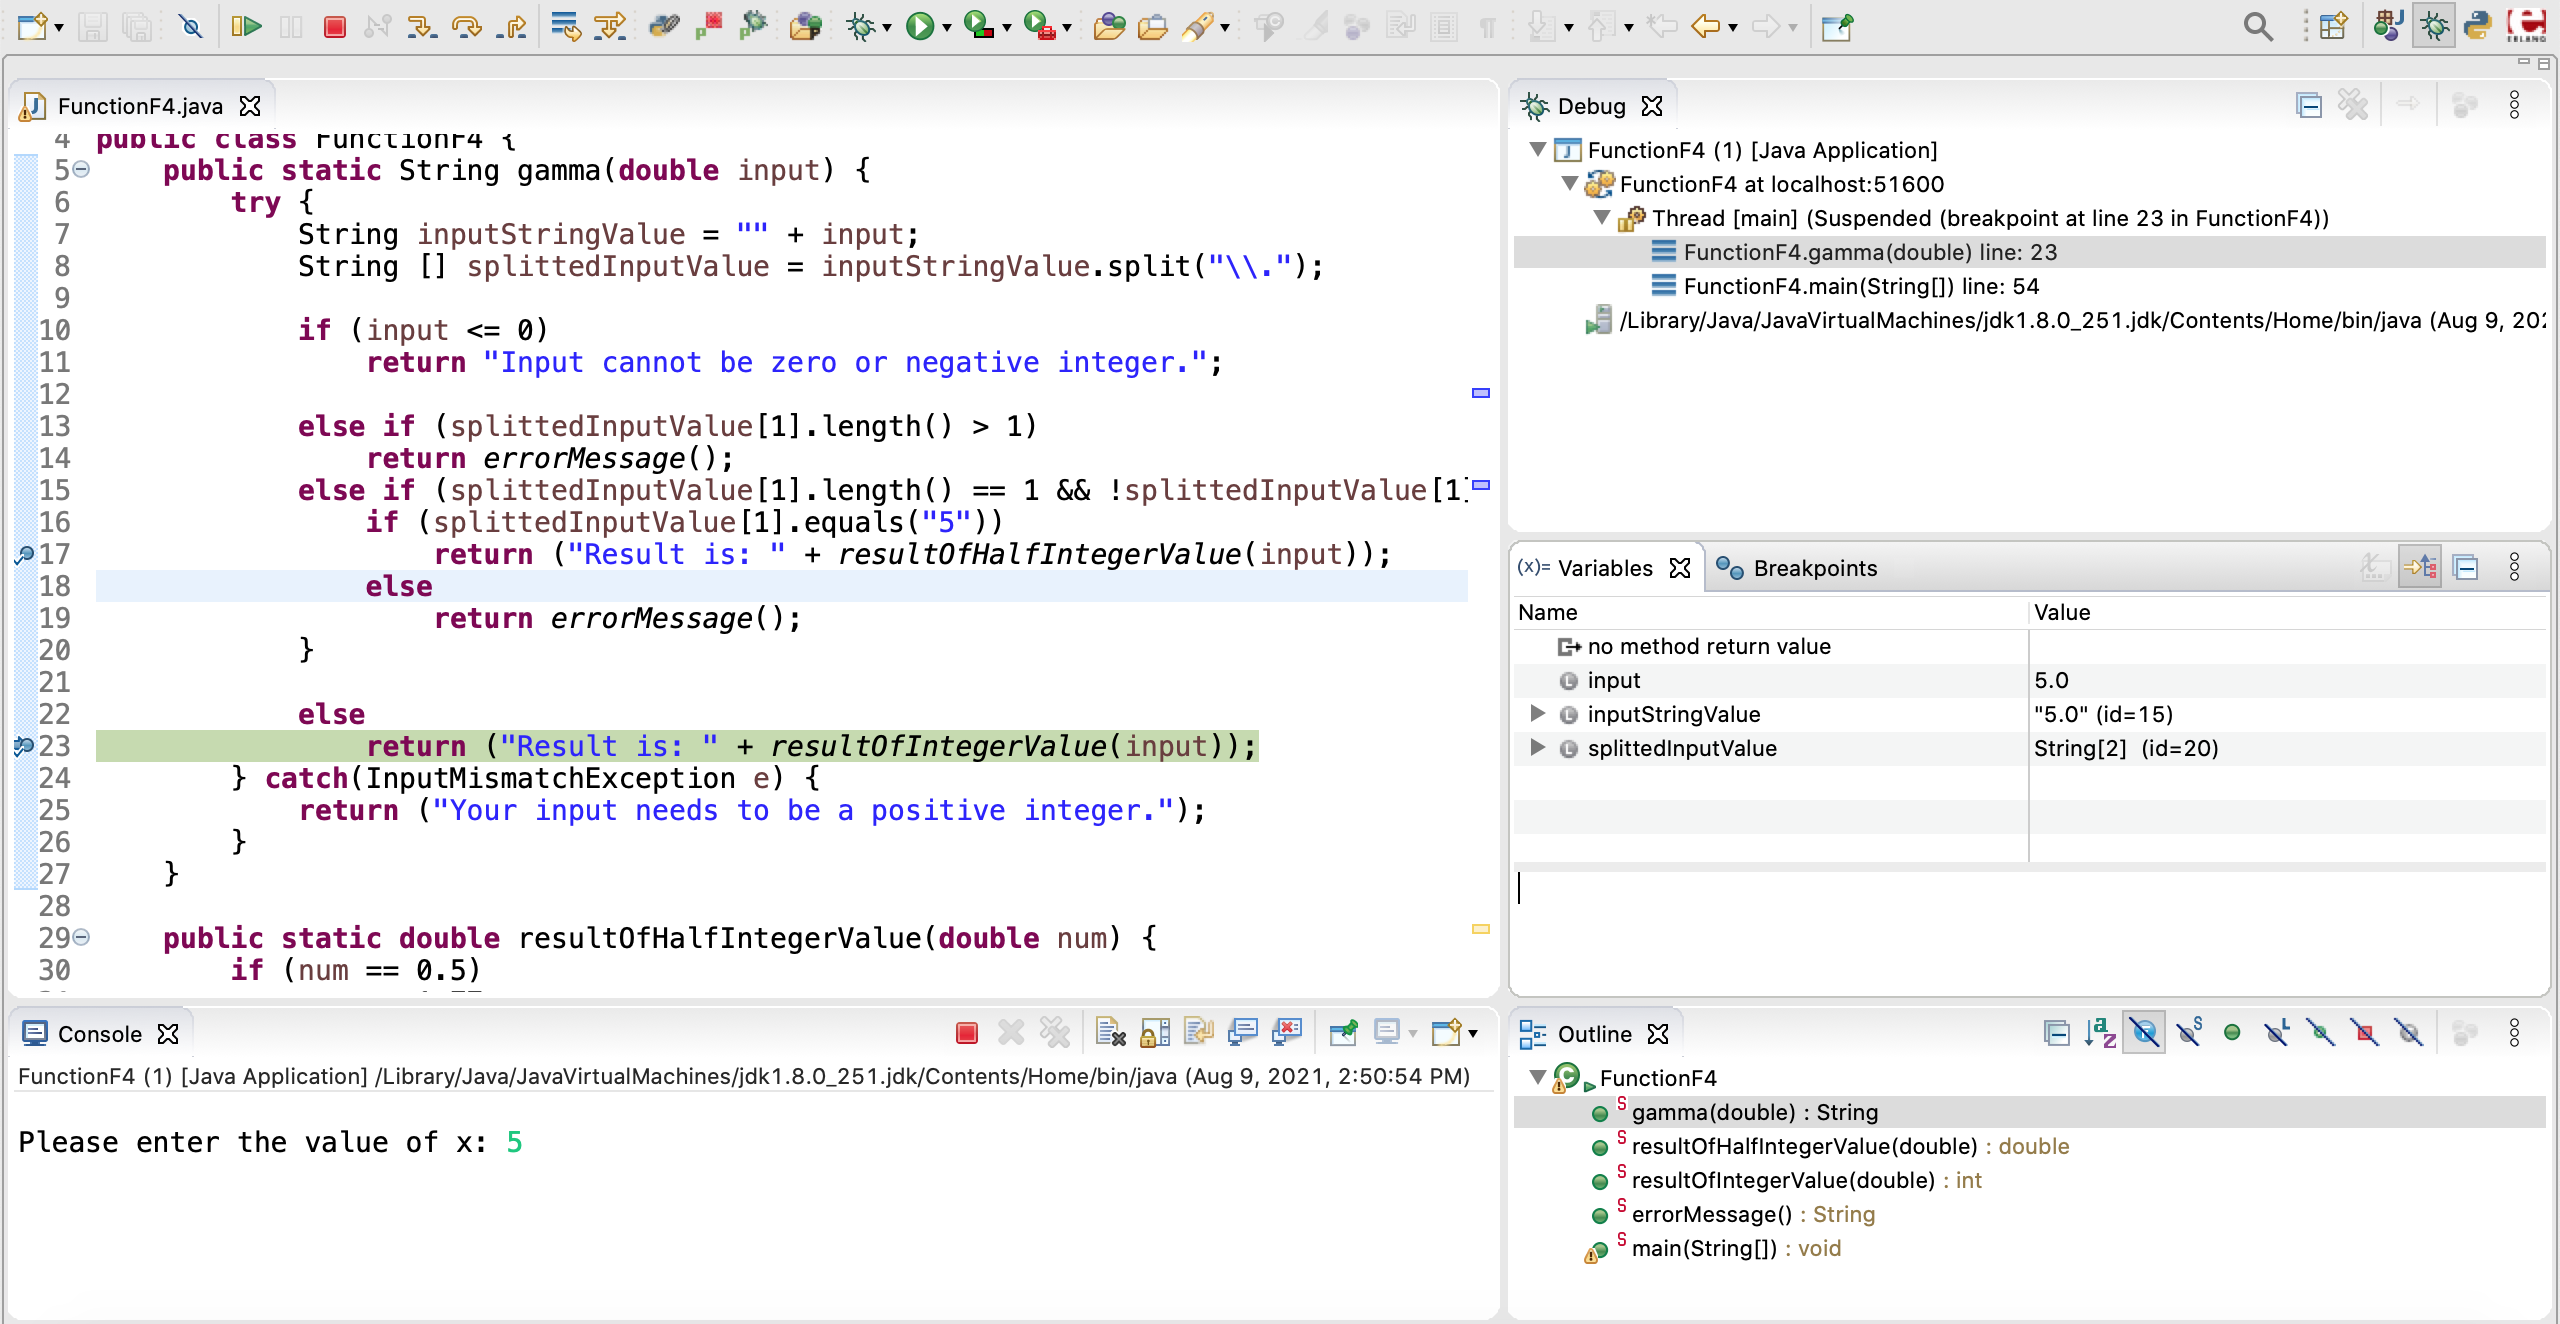
\includegraphics[width=16cm, height=7cm]{debugger.png}
    \subsection{Advantages}
    \begin{itemize}
        \item It is free and open source.
        \item It is easy to use – setting breakpoints, executing code line by line, and inspecting the value of variables and expressions.
        \item It also supports other programming languages than Java for investigating and fixing problems with the code.
    \end{itemize}
    
    \subsection{Disadvantages}
    \begin{itemize}
        \item It is usually slower than other debuggers like Visual Studio.
        \item The independent processes cannot be attached to the eclipse debugger to debug.
    \end{itemize}
\end{document}
